\chapter{Estado del arte}\label{cap.estado}
En este capítulo se presenta el estado del arte sobre la predicción mediante redes neuronales de aprendizaje profundo. Se exponen distintos trabajos enfocados en las estructuras neuronales para la predicción y la realización de esta tarea con secuencias de valores, así como otros que ponen el foco en la predicción con secuencias de imágenes en un vídeo. También se presenta la infraestructura \textit{software} y \textit{hardware} utilizada en el desarrollo del trabajo.\\

\section{Estructuras neuronales para la predicción}
Antes de llegar al conocimiento y el uso de las \acrshort{rnn} y las \acrshort{lstm}, estructuras dinámicas utilizadas en este trabajo, se desarrollaron varias investigaciones que permitían, en cierta forma, predecir un elemento en una secuencia a partir de elementos previos de la misma secuencia haciendo uso de estructuras de naturaleza estática, es decir, no recurrentes.\\

En 1990, Elman realizó un estudio sobre la estructura temporal con el que logró dotar de cierta memoria a las estructuras de aprendizaje~\cite{elman1990finding}. En este artículo, se llega a importantes conclusiones que permitieron avanzar en el desarrollo de estructuras dinámicas que faciliten la tarea de predicción: 

\begin{itemize}
    \item Algunos problemas pueden cambiar el enfoque por el hecho de incluir en ellos la variable temporal.
    \item La señal de error variable en el tiempo puede ser de ayuda para establecer la estructura temporal.
    \item Aumentar las dependencias secuenciales en una tarea no tiene por qué implicar un peor rendimiento.
    \item La representación tiempo-memoria depende de la tarea que se quiera llevar a cabo.
    \item Las representaciones de los datos no tienen por qué tener una estructura concreta.
\end{itemize}

El trabajo de Elman fue muy utilizado en estudios posteriores que se centran en la predicción con secuencias temporales mediante estructuras dinámicas. Por ejemplo, en el año 1996, Koskela \textit{et al.}~\cite{koskela1996time} desarrollaron un trabajo en el que se comparaban tres tipos de redes para la tarea de predicción, obteniendo resultados muy similares entre las redes Elman y los \acrshort{mlp}. Para el uso de los \acrshort{mlp} se modifica su estructura introduciendo las entradas retardadas de manera sucesiva, logrando así obtener un comportamiento dinámico. Los resultados obtenidos en el estudio muestran que la el algoritmo de aprendizaje es un factor más importante que el modelo de red neuronal utilizado. Además, a pesar de ser mucho más sencillo, el modelo MLP obtiene un rendimiento muy bueno en varias de las series, reduciendo sustancialmente el tiempo de entrenamiento.\\

También en los años 90, Kevin J.Lang \textit{et al.}~\cite{LANG199023} introdujeron una nueva forma para dotar de memoria a las estructuras: las Redes Neuronales de Retardo Temporal (TDNN). Se trata de redes multicapa realimentadas cuyas neuronas ocultas y de salida se replican en el tiempo, de forma que las salidas de una capa se almacenan durante varios instantes de tiempo y, posteriormente, alimentan a la siguiente capa. La topología de este tipo de redes se incluye dentro de un \acrshort{mlp}, donde cada conexión sináptica está representada por un filtro de respuesta finita.\\

Finalmente, se llega a las \acrshort{rnn}. Estas redes fueron inventadas en la década de los 80, con el desarrollo por John Hopfield de una red que lleva su mismo nombre. Este tipo de redes se usan como sistemas de memoria asociativa con unidades binarias. Están diseñadas para converger a un mínimo local, pero dicha no está garantizada~\cite{Hopfield:2007}. Tras esta primera \acrshort{rnn} se fueron desarrollando muchas otras, como las \acrshort{lstm}, cuyo concepto se introdujo en el año 1997 por Sepp Hochreiter y Jürgen Schmidhuber~\cite{hochreiter1997long}. En este estudio se analiza la transmisión del error hacia atrás y se desarrolla una nueva arquitectura formada por una capa de entrada, una oculta y la capa de salida. La capa oculta está completamente conectada y la forman un conjunto de celdas de memoria y sus correspondientes puertas, que se encargan de evitar un conflicto con los pesos de entrada. La celda de memoria es el elemento principal de estas redes y pueden ser agrupadas en bloques que compartan las puertas de entrada y de salida, facilitando el almacenamiento de la información. En la Figura~\ref{fig.lstm_net} se muestra una red de este tipo que consta de 8 neuronas en la capa de entrada, cuatro en la salida, y dos celdas de memoria en la oculta.\\

\begin{figure}[H]
	\begin{center}
		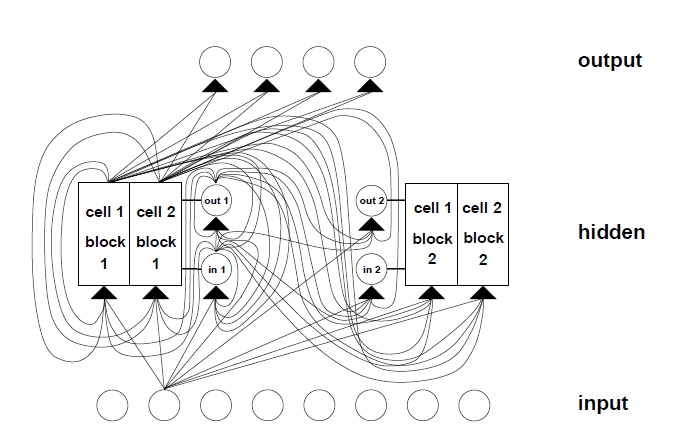
\includegraphics[width=0.7\textwidth]{ figures/estadoarte/lstm_net.PNG}
		\caption{Red LSTM. Imagen obtenida de~\cite{hochreiter1997long}.
		}
		\label{fig.lstm_net}
	\end{center}
\end{figure}
\vspace{-10pt}

Los trabajos expuestos anteriormente dan lugar a la definición de una serie de estructuras dinámicas que permiten abordar con aprendizaje profundo la tarea de la predicción.

\section{Predicción de valores}
El uso de secuencias de valores para la predicción mediante el uso de \acrshort{rna} marca la primera vía de investigación en esta tarea. Así mismo, actualmente es la vía más desarrollada y que presenta muchos de los ejemplos existentes.\\

En el año 2002, miembros del \textit{Institute of Electrical and Electronics Engineers} llevaron a cabo un estudio~\cite{arimaprices} en el se desarrolla un método para predecir los precios de la electricidad al día siguiente según los modelos \acrfull{arima}. Este tipo de modelos se basan en el uso de una serie de procesos estocásticos para analizar series de tiempo, y fue introducida por Box y Jenkins~\cite{box1994series}. El estudio propone dos modelos de este tipo para predecir los precios en cada hora para los mercados eléctricos de España y California, que alcanzan resultados satisfactorios. De entre las conclusiones a las que llega esta investigación cabe destacar que el histórico temporal necesario para realizar la predicción de una forma satisfactoria varía según el mercado, siendo mayor en el español. Además, se plantea el uso de variables explicativas que permiten mejorar los resultados en aquellos meses con una alta correlación entre la producción hidroeléctrica disponible y el precio de la electricidad.\\

En relación con el trabajo anterior, otro estudio que hace uso de los modelos \acrshort{arima} es el desarrollado por G. Peter Zhang~\cite{arimann}, en el que se propone combinar dichos modelos con las \acrshort{rna} para distintas secuencias de valores. El desarrollo de un modelo híbrido viene motivado por la naturaleza combinada de las series temporales: es difícil determinar si una serie de tiempo se genera a partir de un proceso subyacente lineal o no lineal. Con un modelo híbrido se tiene la flexibilidad para modelar una variedad de problemas aprovechando la fuerza en la correlación lineal de \acrshort{arima} y en la no lineal de las \acrshort{rna}. El estudio concluye que, efectivamente, un modelo híbrido ofrece mejores prestaciones que cada modelo por separado, sin embargo la diferencia no es demasiado significativa, según se muestra en la Figura~\ref{fig.arimann}.\\

\begin{figure}[H]
	\begin{center}
		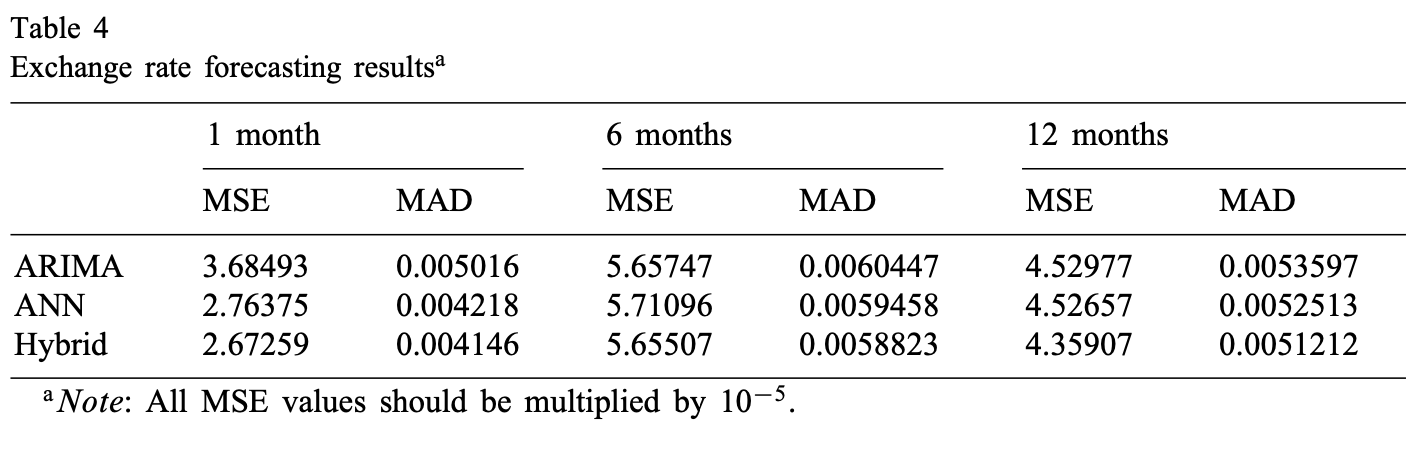
\includegraphics[width=0.85\textwidth]{ figures/estadoarte/ARIMA+NN.png}
		\caption{Resultados comparativos de \acrshort{arima}, \acrshort{rna} y \acrshort{arima}+\acrshort{rna}. Imagen obtenida de~\cite{arimann}.
		}
		\label{fig.arimann}
	\end{center}
\end{figure}
\vspace{-10pt}

Un estudio similar es el desarrollado por un grupo de investigadores japoneses en el año 2015~\cite{dbnARIMA}. En dicho trabajo se combina los modelos \acrshort{arima} con un tipo de red estocástica llamada \acrfull{rbm} seguida de un \acrshort{mlp}. En la Figura~\ref{fig.dbnarima} se muestra el flujo del modelo propuesto, en el que se integran los dos modelos. Se sitúa el foco de la investigación en cómo afecta el orden de ambos modelos en la predicción de distintos valores económicos. El estudio concluye que el orden adecuado depende del tipo de datos con el que se esté trabajando.
\vspace{10pt}
\begin{figure}[H]
	\begin{center}
		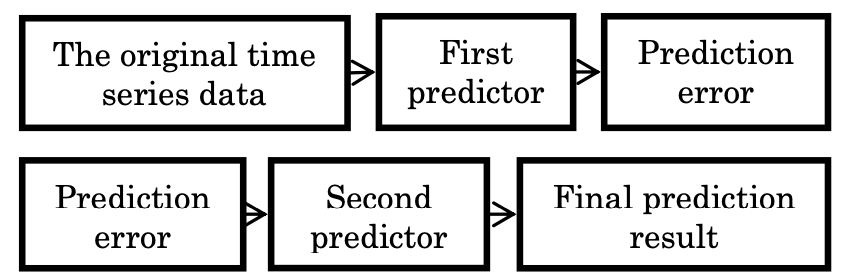
\includegraphics[width=0.5\textwidth]{ figures/estadoarte/flujo_dbn.png}
		\caption{Diagrama de flujo del estudio~\cite{dbnARIMA}.
		}
		\label{fig.dbnarima}
	\end{center}
\end{figure}
\vspace{-10pt}

Respecto al uso de redes recurrentes, Erol Egrioglu, Ufuk Yolcu, Cagdas Hakan Aladag y Eren Basen desarrollan un estudio en el que se propone una arquitectura combinada de \acrshort{rnn} y \acrshort{rna}~(RMNM-ANN)~\cite{multiplicative}. La \acrshort{rnn} propuesta se basa en el modelo de neuronas multiplicativas que se caracterizan por el uso de funciones de agregación multiplicativas en lugar de aditivas. El nuevo modelo, representado en la Figura~\ref{fig.rmnm-ann}, puede producir variables de error rezagadas y utilizarlas como entradas gracias a su estructura de retroalimentación recurrente, y hace uso de una única neurona en la capa oculta de la \acrshort{rna}. El modelo propuesto se aplicó para estimar la cantidad de dióxido de carbono medida mensualmente en Ankara entre marzo de 1995 y abril de 2006, proporcionando mejores resultados que otros modelos de la literatura.

\vspace{10pt}
\begin{figure}[H]
	\begin{center}
		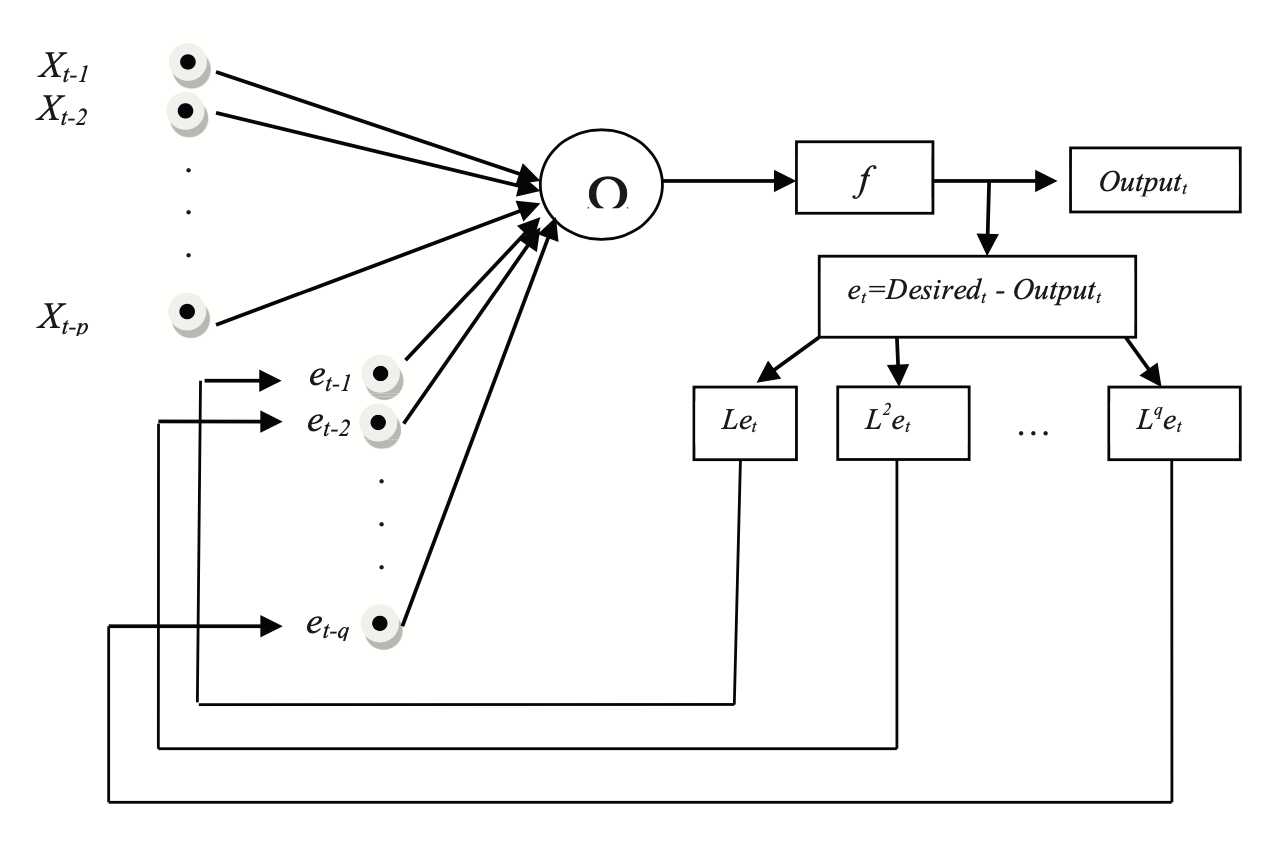
\includegraphics[width=0.51\textwidth]{ figures/estadoarte/rmnm-ann.png}
		\caption{Estructura de RMNM-ANN~\cite{multiplicative}.
		}
		\label{fig.rmnm-ann}
	\end{center}
\end{figure}
\vspace{-10pt}

Algunos estudios han utilizado una combinación de datos de distinta naturaleza para lograr una predicción más precisa. A modo de ejemplo, un artículo de 2018  combina datos temporales con información en forma de texto no estructurado para estimar la demanda de taxi en la ciudad de Nueva York~\cite{taxi}. Para ello se proponen dos estructuras, utilizando una red para el texto y otra para la información temporal y que conjuntamente logran superar de modo significativo a otros métodos populares. La principal diferencia entre ambas estructuras se encuentra en la red utilizada para el procesamiento de la información temporal, que puede ser \acrshort{lstm}~(véase la Figura~\ref{fig.taxi}) o \textit{fully connected}.

\vspace{10pt}
\begin{figure}[H]
	\begin{center}
		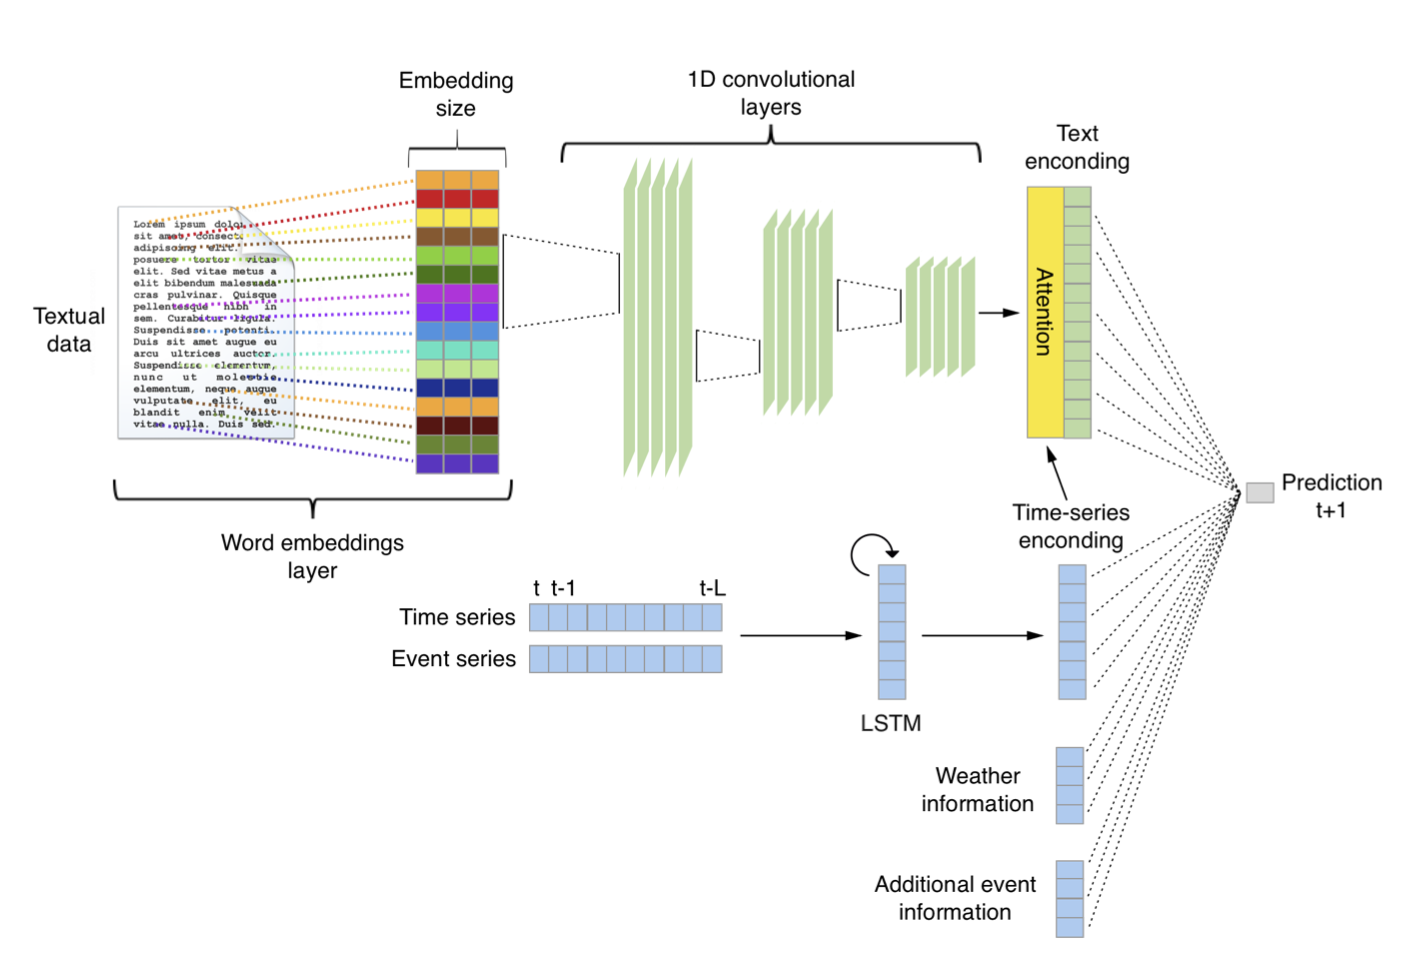
\includegraphics[width=0.95\textwidth]{ figures/estadoarte/taxi.png}
		\caption{Estructura propuesta por~\cite{taxi} con \acrshort{lstm}.
		}
		\label{fig.taxi}
	\end{center}
\end{figure}
\vspace{-10pt}

Finalmente, en cuanto al seguimiento de trayectorias, se han llevado a cabo varios estudios. En el año 2016, se presentó en un artículo la red \textit{SocialLSTM}, cuyo objetivo es lograr es predecir la dinámica del movimiento de peatones en escenas abarrotadas. Esta red es capaz de predecir de forma conjunta las trayectorias de todas las personas que aparecen en una escena teniendo en cuenta las reglas de sentido común y las convenciones sociales que los humanos utilizan mientras se desplazan. Se utiliza una \acrshort{lstm} independiente para cada trayectoria y, posteriormente, se conectan todas ellas a través de una capa de agrupación social (\textit{S-pooling}), compartiendo información entre sí. En la Figura~\ref{fig.socialstm} se muestra la estructura de la red propuesta. El método propuesto logra superar a los métodos de vanguardia en dos conjuntos de datos públicos~(ETH y UCY). Además, es capaz de predecir con éxito varios comportamientos no lineales que surgen de interacciones sociales. 

\vspace{10pt}
\begin{figure}[H]
	\begin{center}
		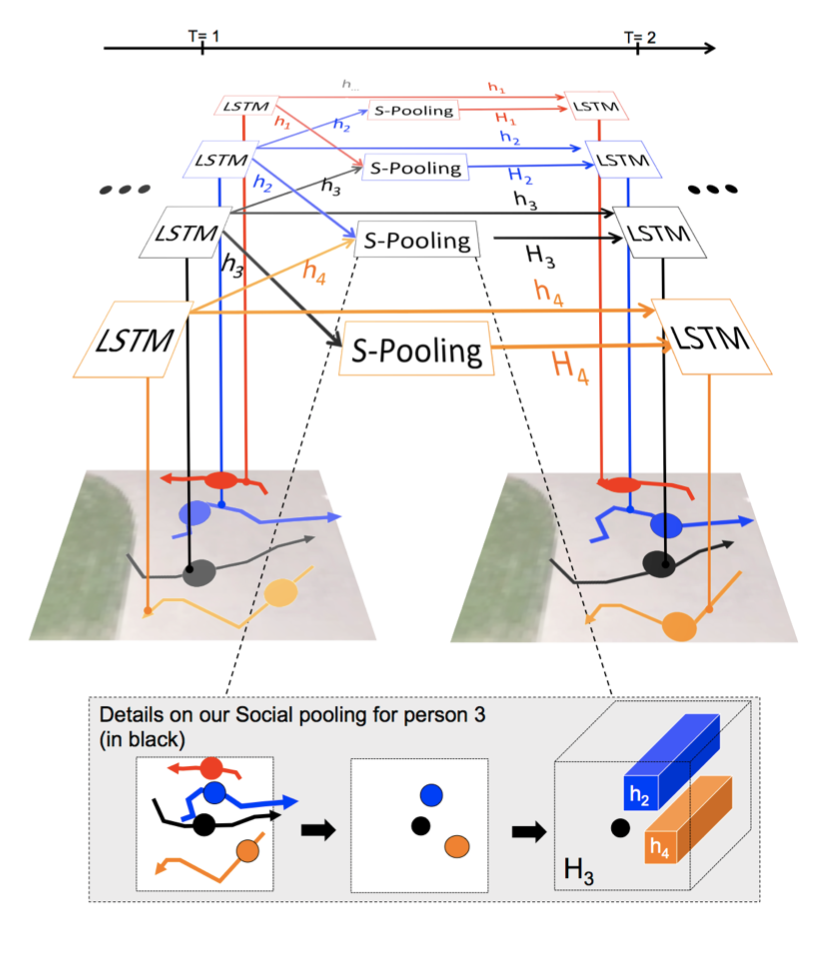
\includegraphics[width=0.7\textwidth]{ figures/estadoarte/sociallstm.png}
		\caption{Estructura de SocialLSTM~\cite{sociallstm}.
		}
		\label{fig.socialstm}
	\end{center}
\end{figure}
\vspace{-10pt}



Otro estudio en relación con trayectorias, en esta ocasión de vehículos~\cite{vehicletrajectory}, se publica en el 2018 y se basa en la arquitectura de red neuronal del codificador-decodificador \textit{lstm}\footnote{\url{https://machinelearningmastery.com/encoder-decoder-long-short-term-memory-networks/}}. El sistema propuesto, mostrado en la Figura~\ref{fig.vehicletrajectory}, se basa en el análisis de varias observaciones pasadas del vehículo por el codificador para que el decodificador genere un número \textit{K} de posibles trayectorias a seguir. Este método es capaz de lograr una mejora significativa con respecto a los métodos existentes en términos de precisión de predicción, al mismo tiempo que puede generar la secuencia completa de la trayectoria predicha.

\vspace{10pt}
\begin{figure}[H]
	\begin{center}
		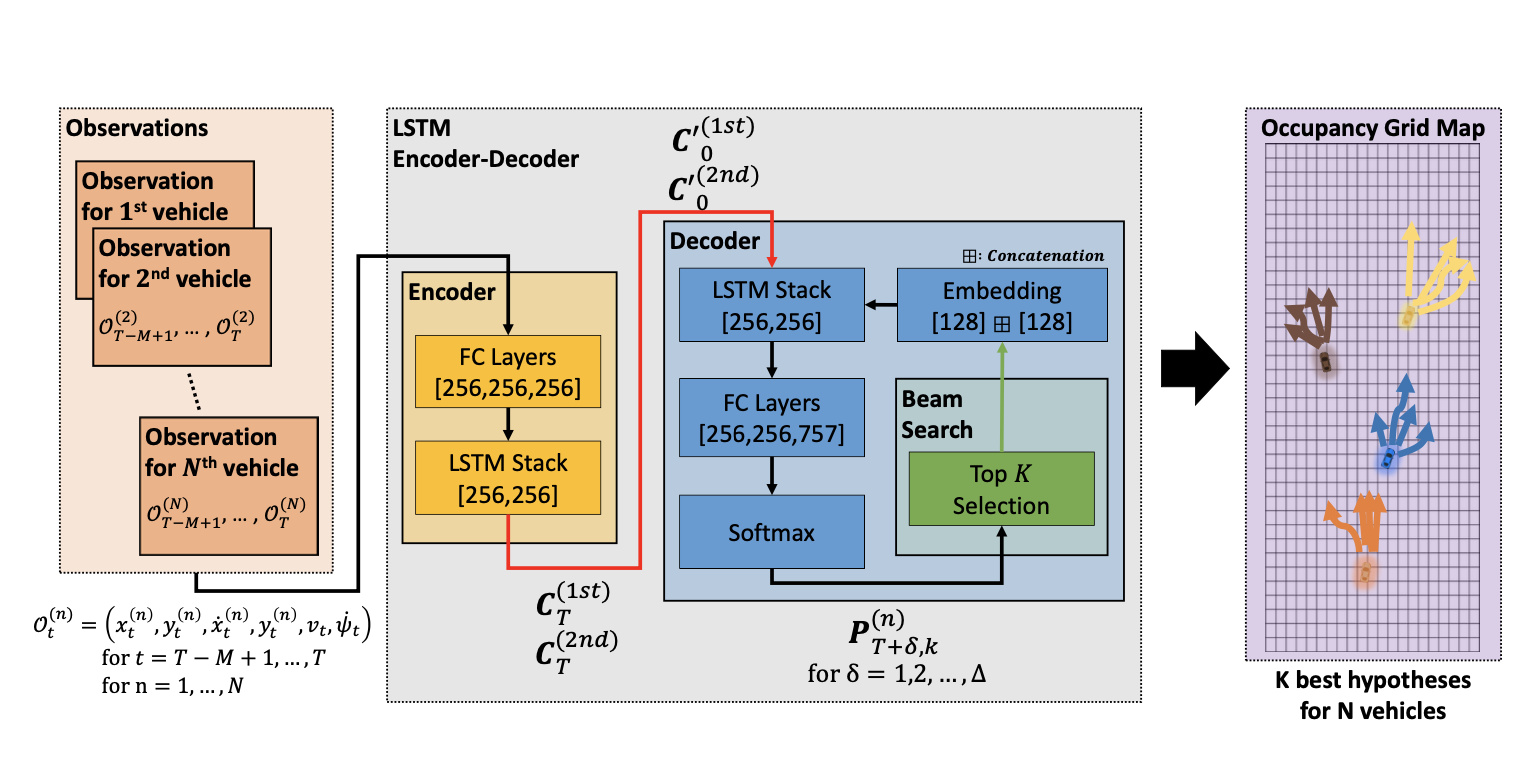
\includegraphics[width=0.95\textwidth]{ figures/estadoarte/vehicle_trajectory.png}
		\caption{Estructura propuesta por~\cite{vehicletrajectory}.
		}
		\label{fig.vehicletrajectory}
	\end{center}
\end{figure}
\vspace{-10pt}

\section{Predicción en imágenes}
La investigación en la tarea de predicción con secuencias de imágenes o de vídeo está menos desarrollada, puesto que surge más tarde que para las secuencias numéricas.\\

Uno de los campos en los que se han realizado estudios de predicción con imágenes es el de los videojuegos. En el año 2015 se publica un artículo~\cite{actiongames} que propone dos estructuras, mostradas en la Figura~\ref{fig.games_nets}, novedosas hasta el momento para la predicción de fotogramas que dependen de las acciones del jugador. Los resultados, tanto cualitativos como cuantitativos, muestran que ambas redes son capaces de predecir fotogramas visualmente realistas y útiles para el control del juego, con una separación temporal~(\textit{gap}) de 100 pasos en varios juegos de Atari de distinto dominio. Se trata de uno de los primeros artículos que muestra buenas predicciones en los juegos de Atari.\\

\vspace{10pt}
\begin{figure}[H]
	\begin{center}
		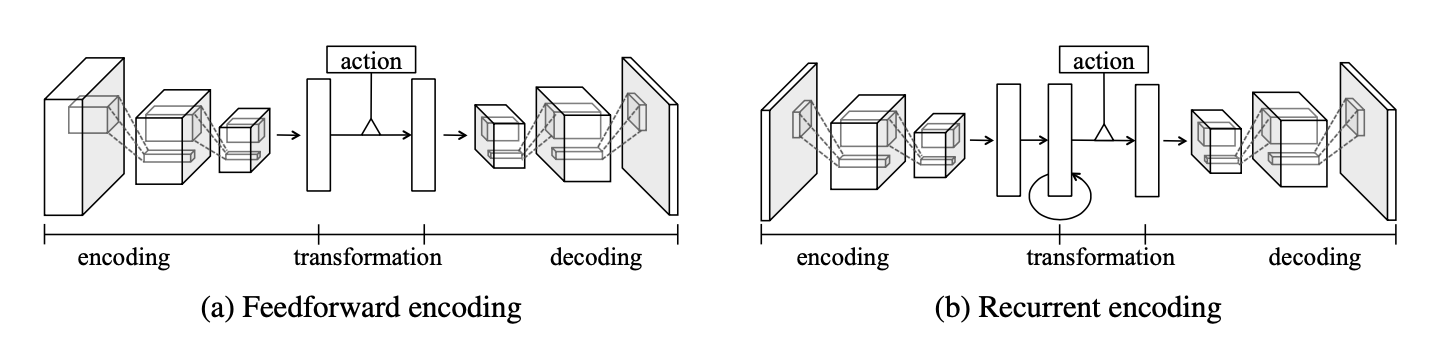
\includegraphics[width=0.95\textwidth]{ figures/estadoarte/games_nets.png}
		\caption{Estructuras propuestas en~\cite{actiongames}.
		}
		\label{fig.games_nets}
	\end{center}
\end{figure}
\vspace{-10pt}

Otro campo de estudio es la predicción de secuencias de vídeo, anticipándose a las acciones que sucederán en la secuencia. Un ejemplo de ello es el artículo propuesto por Carl Vondrick, Hamed  Pirsiavash y Antonio Torralba, que se centra en dicha predicción mediante aprendizaje no supervisado~\cite{unlabeledvideo}. Se propone la estructura definida en la Figura~\ref{fig.unlabeled_net}, entrenada con más de 600 horas de vídeo de \textit{YouTube} con diferentes temáticas. Con las predicciones obtenidas realizan una clasificación de la acción que se está desarrollando en la escena, obteniendo resultados bastante satisfactorios aunque con margen de mejora.

\vspace{10pt}
\begin{figure}[H]
	\begin{center}
		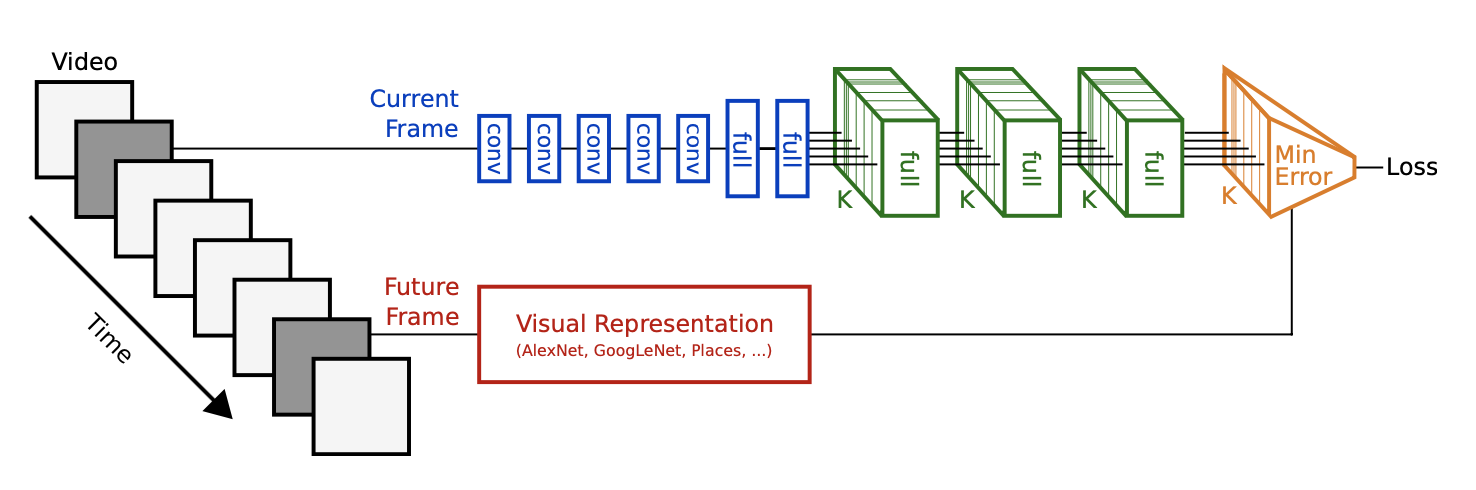
\includegraphics[width=0.95\textwidth]{ figures/estadoarte/unlabeled_net.png}
		\caption{Estructura propuesta en~\cite{unlabeledvideo}.
		}
		\label{fig.unlabeled_net}
	\end{center}
\end{figure}
\vspace{-10pt}

En en año 2018 se publica un estudio que propone la descomposición del movimiento y el contenido para manejar de forma efectiva la evolución los píxeles en los vídeos~\cite{descompose}. El modelo propuesto~(MCnet), mostrado en la Figura~\ref{fig.descompose}, se basa en un codificador-decodificador con \acrshort{cnn} y una \acrshort{lstm} convolucional que obtiene la predicción a nivel de píxel. Debido a la separación entre movimiento y contenido, la predicción se obtiene convirtiendo el contenido extraído en el contenido del siguiente fotograma mediante las características de movimiento identificadas, simplificando la tarea. Para evaluar la red y compararla con otras estructuras han empleado los conjuntos de datos KTH, Weizmann action y UCF-101, que están formados por vídeos de actividad de personas. La estructura propuesta es considerada una de las primeras arquitecturas que realizan la separación de movimiento y contenido en la predicción a nivel de píxeles en vídeos naturales.\\

\vspace{10pt}
\begin{figure}[H]
	\begin{center}
		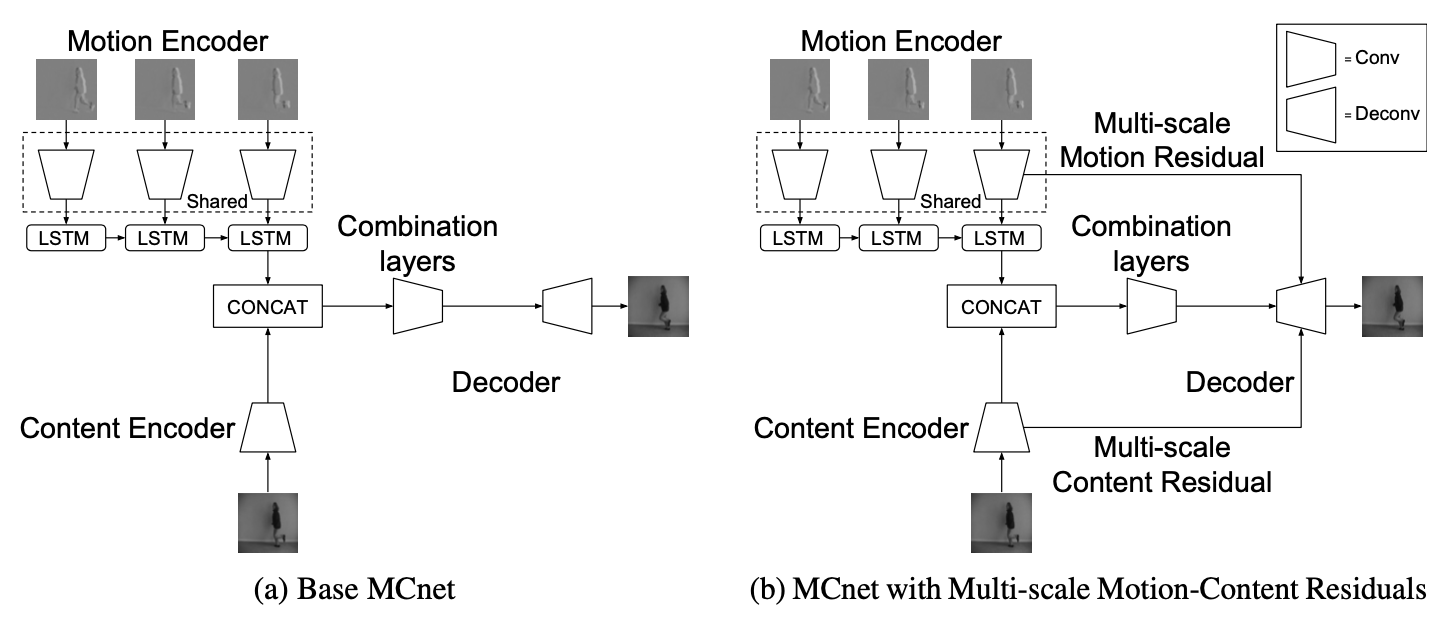
\includegraphics[width=0.95\textwidth]{ figures/estadoarte/descompose.png}
		\caption{Estructura de red MCnet~\cite{descompose}.
		}
		\label{fig.descompose}
	\end{center}
\end{figure}
\vspace{-10pt}

En el año 2019, Jason Y. Zhang, Panna Felsen, Angjoo Kanazawa y Jitendra Malik llevaron a cabo un estudio para predecir el movimiento 3D de una persona a partir de una secuencia de vídeo~\cite{3d}. Es uno de los primeros enfoques que tratan de predecir una malla 3D a partir de una serie de fotogramas, por lo que el margen de mejora es todavía bastante amplio. Este modelo~(PHD) centra su atención en acciones periódicas como el caminar, lanzar a los bolos o realizar un ejercicio de gimnasio. En la Figura~\ref{fig.3d} se muestra un ejemplo de funcionamiento. 

\vspace{10pt}
\begin{figure}[H]
	\begin{center}
		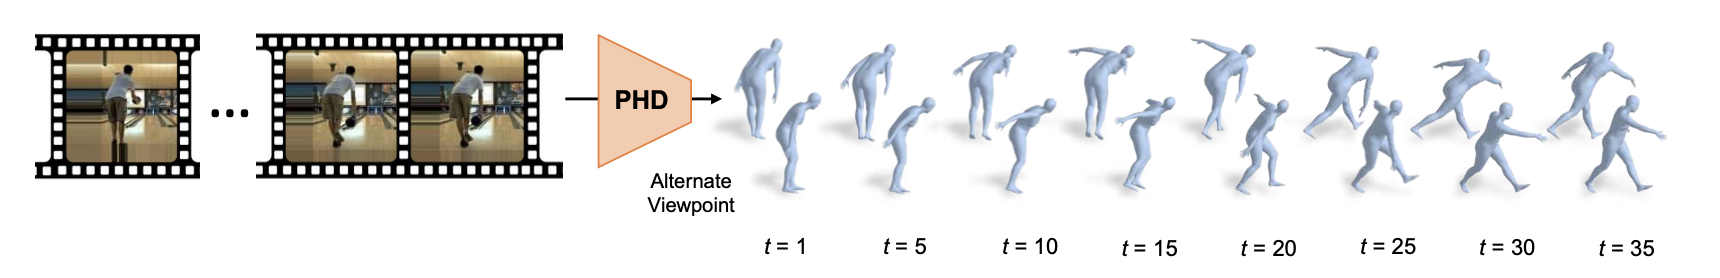
\includegraphics[width=1\textwidth]{ figures/estadoarte/3D-func.png}
		\caption{Funcionamiento de PHD~\cite{3d}.}
		\label{fig.3d}
	\end{center}
\end{figure}
\vspace{-10pt}

La arquitectura definida se basa en modelos autorregresivos y no necesita de vídeos etiquetados en 3D, se puede entrenar con vídeos que sólo dispongan de anotaciones 2D. El modelo desarrollado en este estudio, mostrado en la Figura~\ref{fig.3d_net}, está formado por cuatro partes:
\begin{itemize}
    \item Una \textit{Resnet} que se encarga de extraer las características de cada fotograma.
    \item Un codificador temporal causal que aprende una ``tira de película'', es decir, una representación latente de la dinámica humana en 3D.
    \item Un regresor 3D que puede leer la malla 3D de la tira de película.
    \item Un modelo autorregresivo en el espacio latente que toma las tiras de películas pasadas para predecir las películas futuras, capturando así la dinámica humana.
\end{itemize}

\vspace{10pt}
\begin{figure}[H]
	\begin{center}
		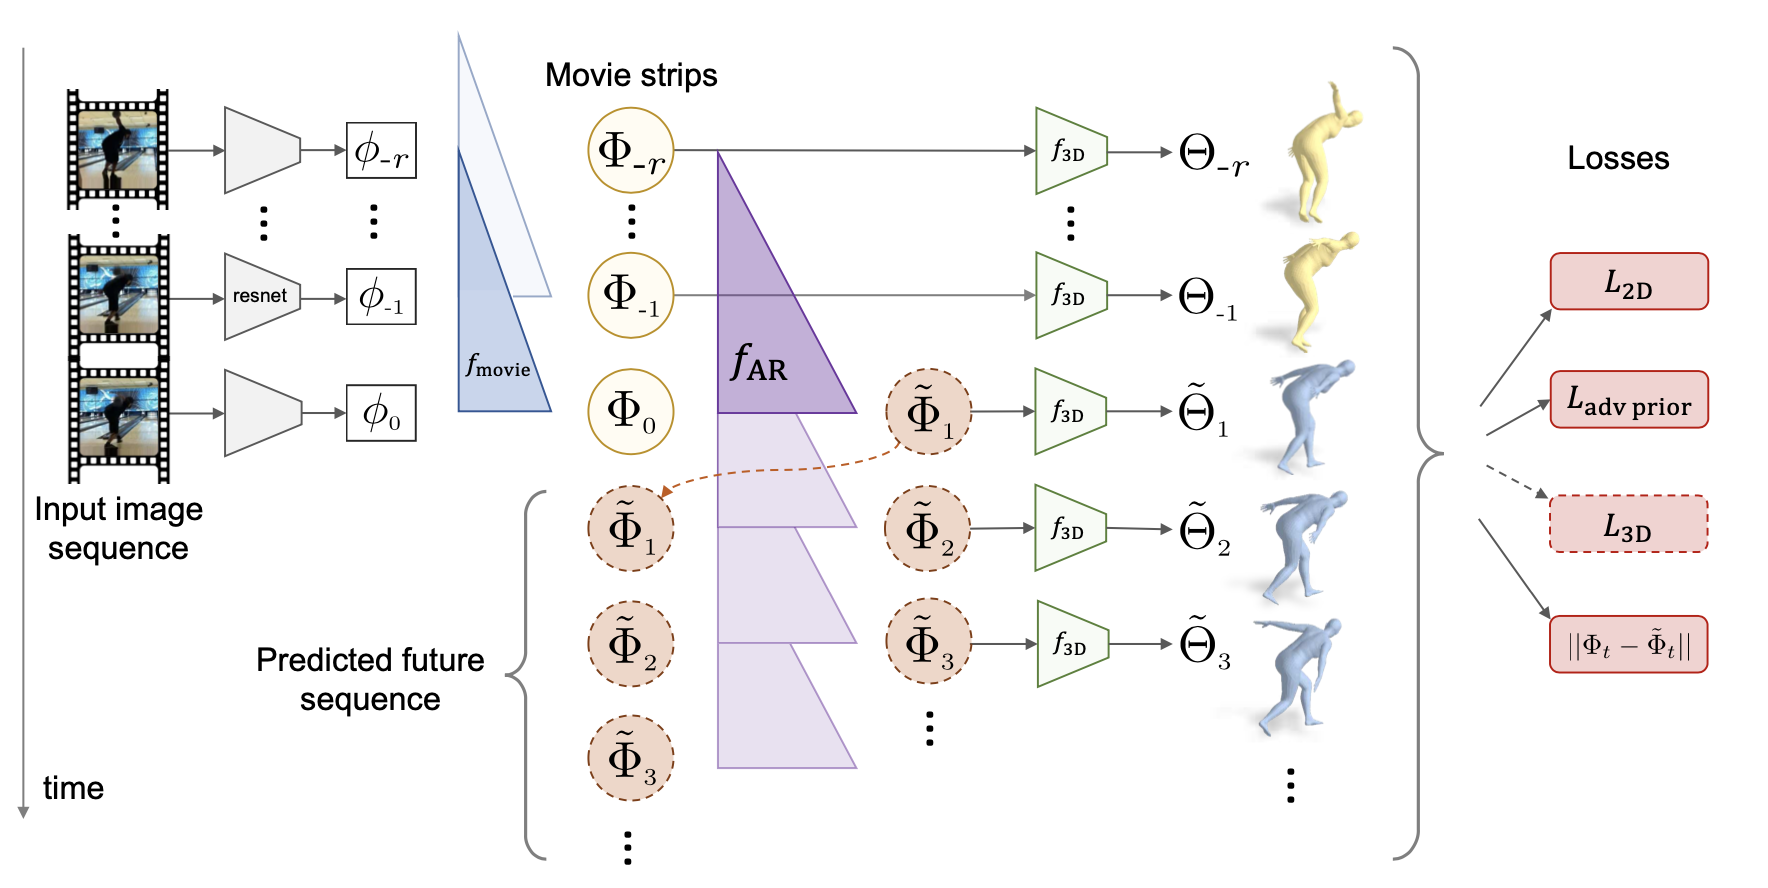
\includegraphics[width=0.95\textwidth]{ figures/estadoarte/3D-net.png}
		\caption{Estructura de red PHD~\cite{3d}.}
		\label{fig.3d_net}
	\end{center}
\end{figure}
\vspace{-10pt}

Finalmente, uno de los estudios más recientes~\cite{photorealistic} trata de obtener la predicción del fotograma lo más nítida y realista posible, evitando las distorsiones que generan otros métodos de predicción. Para ello se hace uso de la estructura definida en la Figura~\ref{fig.real-net}, una red residual profunda con arquitectura jerárquica donde cada capa hace una predicción del estado futuro a diferentes resoluciones espaciales para después fusionarlas a través de conexiones de arriba hacia abajo.

\vspace{10pt}
\begin{figure}[H]
	\begin{center}
		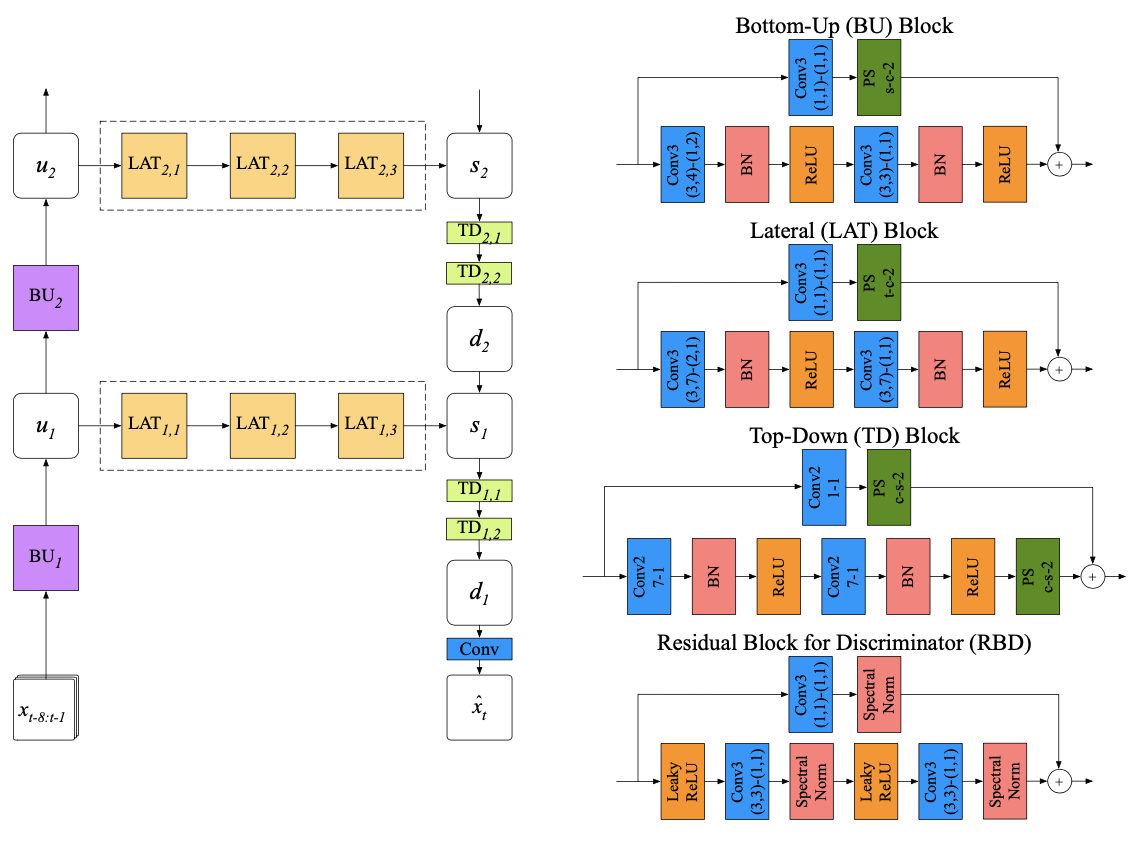
\includegraphics[width=0.85\textwidth]{ figures/estadoarte/Real-net.png}
		\caption{Estructura propuesta en~\cite{photorealistic}.}
		\label{fig.real-net}
	\end{center}
\end{figure}
\vspace{-10pt}

El modelo propuesto supera cuantitativamente las líneas del estado del arte en la predicción de fotogramas futuros y es capaz de generar fotogramas con detalles más finos y texturas que son perceptualmente más realistas, según se muestra en la Figura~\ref{fig.real-func}.

\vspace{10pt}
\begin{figure}[H]
	\begin{center}
		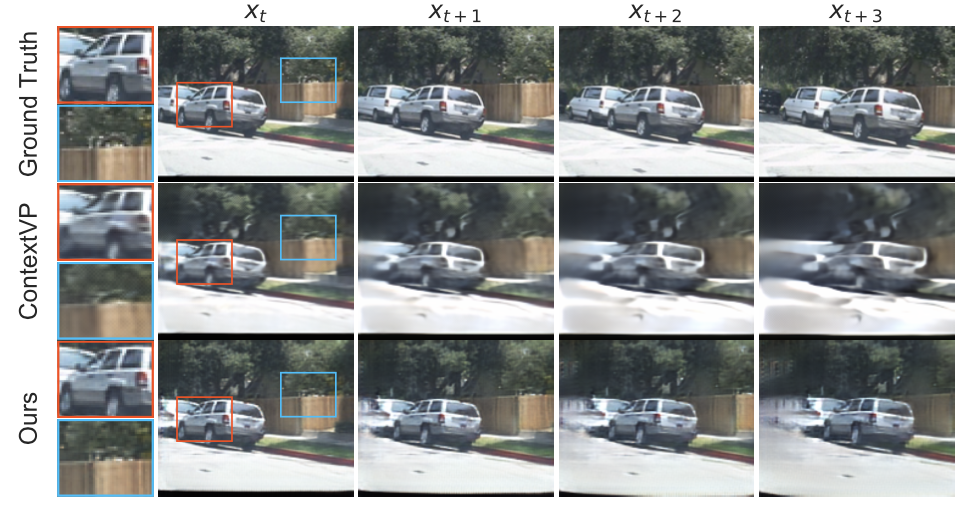
\includegraphics[width=0.85\textwidth]{ figures/estadoarte/Real-func.png}
		\caption{Resultados de estructura propuesta en~\cite{photorealistic}.}
		\label{fig.real-func}
	\end{center}
\end{figure}
\vspace{-10pt}

\section{Infraestructura utilizada}
Esta sección describe los elementos \textit{software} y \textit{hardware} utilizados en el desarrollo de este trabajo. Se explica el lenguaje de programación empleado, las herramientas \textit{software} necesarias, y el servidor en el que se han ejecutado todos los experimentos.

\subsection{Lenguaje Python}
Python\footnote{\url{https://www.python.org}} es un lenguaje de programación orientado a objetos, interpretado e interactivo que combina una alta potencia con una sintaxis muy clara. Esta sencillez en la sintaxis hace que sea fácil de aprender. Además la comunidad de desarrolladores proporciona conferencias, documentación y listas de correo que facilitan su aprendizaje.\\

La potencia de este lenguaje viene dada por la fácil combinación de la biblioteca estándar con miles de módulos de terceros que permite aumentar casi infinitamente el rango de posibilidades de sus aplicaciones. Además, puede ser utilizado como lenguaje de extensión para aplicaciones escritas en otros lenguajes que necesitan interfaces de automatización o \textit{scripts} fáciles de usar. Todo esto hace que su uso se haya extendido en las distintas aplicaciones de \acrshort{ia}. Es un lenguaje de código abierto que permite su libre uso y distribución, cuya licencia está administrada por la \textit{``Python Software Foundation''}.\\

Actualmente, la versión de Python más reciente es la 3.8.6,  lanzada el 24 de septiembre de 2020. Sin embargo, en la realización de este trabajo se ha utilizado la versión 3.6.9, pues era la última en el momento de comenzar el desarrollo.

\subsection{Biblioteca OpenCV}
OpenCV (\textit{Opne Source Computer Vision Library})\footnote{\url{https://opencv.org}} es una librería de código abierto para realizar tareas de \acrshort{va} y aprendizaje automático. Fue creado con el objetivo de facilitar una infraestructura común para diversas aplicaciones de \acrshort{va} y acelerar su uso en productos comerciales.\\

Su uso está muy extendido, pues cuenta con más de 47 mil usuarios en la comunidad y un número aproximado de descargas superior a 18 millones. Su expansión abarca desde grupos de investigación hasta empresas tan potentes como \textit{Google}, y cuenta con algunos usos desplegados como la unión de imágenes en \textit{streetview} o la comprobación de pistas en busca de escombros en Turquía.\\

Presenta interfaces para los lenguajes C++, Java, MATLAB y Python, esta última utilizada en este trabajo. En cuanto a sistemas operativos, es compatible con Windows, Linux, Android y Mac OS. Dispone de más de 2500 algoritmos, clásicos y de última generación, que han sido optimizados y que permiten realizar tareas como la detección de rostros y su identificación, el seguimiento de objetos, la extracción de modelos 3D de los objetos o la búsqueda de patrones.\\

El principal uso de OpenCV en el trabajo se ha centrado en el procesamiento de las imágenes utilizadas para el entrenamiento y la evaluación de las redes mediante tres métodos:

\begin{itemize}
    \item \textbf{\textit{cv2.imwrite(filename, image)}:} Almacena la imagen (\textit{image}) en el fichero (\textit{filename}). Se utiliza en la generación de las imágenes para almacenar las secuencias de imágenes en la base de datos.
    \item \textbf{\textit{cv2.imread(path, flag=0)}:} Lee la imagen almacenada en \textit{path} en escala de grises (\textit{flag=0}). Se utiliza en la lectura las secuencias de imágenes de la base de datos para entrenar o evaluar las distintas redes.
    \item \textbf{\textit{cv2.GaussianBlur(image, (5, 5), 0)}:} Aplica un filtro gaussiano a la imagen para expandir el píxel en una ventana de 5x5. Se utiliza como preprocesamiento de las imágenes en algunos estudios.
\end{itemize}

La versión más reciente de la biblioteca OpenCV en la actualidad es la 4.4.0, mientras que la empleada en este trabajo es la 4.2.0 con su interfaz de Pyhton.

\subsection{Biblioteca Matplotlib}
La librería Matplotlib\footnote{\url{https://matplotlib.org}} está enfocada a la creación de gráficos 2D de matrices en Pyhton. Su origen se sitúa en la emulación de comandos gráficos de MATLAB pero ha desembocado en una biblioteca completamente independiente de este lenguaje que puede ser usada en Python y de forma orientada a objetos. Está escrito principalmente en Python puro, aunque utiliza de forma intensiva la librería Numpy para el tratamiento de matrices, y otros códigos de extensión para un buen rendimiento incluso con matrices grandes. La filosofía de esta biblioteca radica en la capacidad de crear gráficos simples con unos pocos comandos, o tan solo uno.\\

Los usos de Matplotlib son muy variados. En este trabajo se emplean para la representación gráfica de las distintas métricas calculadas para comparar las prestaciones de las diferentes redes. En concreto, se hace uso de dos gráficos:

\begin{itemize}
    \item \textbf{\textit{pyplot.bar}:} Dibuja un diagrama de barras dados un par de vectores \textit{x} e \textit{y} con el mismo número de valores. Permite la modificación de parámetros como el ancho de la barra, su alineación respecto el valor de \textit{x} o el color de la misma.
    \item \textbf{\textit{pyplot.boxplot}:} Dibuja un diagrama de caja y bigotes sobre un conjunto de datos. En este gráfico se representa la caja, con los valores del cuartil inferior al superior de los datos con una línea en la mediana; y los bigotes, que se extienden desde la caja para mostrar el rango de los datos. Además aparecen representados los distintos \textit{outliers} como puntos más allá del final de los bigotes.
\end{itemize}

La versión más reciente de Matplotlib es la 3.3.2, pero en este trabajo se hace uso de la versión 3.1.3.

\subsection{Middleware neuronal Keras}
Keras\footnote{\url{https://keras.io}} es un \textit{middleware} de aprendizaje profundo escrito en Python que se ejecuta sobre la plataforma Tensorflow. Su enfoque de desarrollo se sitúa en lograr una experimentación rápida, pasando de la idea al resultado de una forma fluida. Keras es la API de alto nivel de TensorFlow 2.0 que proporciona abstracciones y bloques de construcción esenciales para desarrollar diversas soluciones de aprendizaje automático con una alta velocidad de iteración.\\

Las estructuras de datos centrales de este \textit{middleware}, sobre las que se entrará en detalle a continuación, son los llamados modelos y capas.

\subsubsection{Modelos en Keras}
Un modelo es una estructura de datos que engloba a otras, las capas, para la creación de redes neuronales de aprendizaje profundo. El tipo de modelo más sencillo definido en Keras, y el utilizado en este trabajo, es el \textit{Sequential()} que apila todas las capas de forma lineal. Para trabajar con estos modelos se utilizan las funciones que se exponen a continuación:

\begin{itemize}
    \item \textbf{\textit{model.add(layer)}:} Se utiliza para añadir una nueva capa (\textit{layer}) al modelo (\textit{model}).
    \item \textbf{\textit{model.compile(...)}:} Sirve para, una vez definida la estructura, configurar la red para el entrenamiento. A esta función se le pueden pasar varios argumentos, siendo empleados en este trabajo dos de ellos:
    \begin{itemize}
        \item \textit{loss}: Define la función de pérdida a optimizar y varía según el experimento a realizar.
        \item \textit{optimizer}: Define el tipo de optimizador a utilizar.
    \end{itemize}
    \item \textbf{\textit{model.fit(...)}:} Entrena el modelo bajo una serie de condiciones. Los parámetros utilizados son:
    \begin{itemize}
        \item \textit{x}: Datos de entrenamiento.
        \item \textit{y}: Etiquetas de entrenamiento.
        \item \textit{batch}\_\textit{size}: Tamaño del lote, número de muestras utilizadas en cada actualización de gradiente.
        \item\textit{epochs}: Número de épocas a entrenar.
        \item \textit{validation}\_\textit{data}: Datos de validación.
        \item \textit{callbacks}: Lista con los objetos para realizar acciones en varias etapas del entrenamiento. En concreto se hace uso de dos de ellos.
        \begin{itemize}
            \item \textit{early}\_\textit{stopping}: Define un criterio de parada en el entrenamiento cuando el valor de la función de \textit{loss} no mejora un número de épocas consecutivas.
            \item \textit{checkpoint}: Guarda el modelo en un punto de control determinado. En este trabajo, se guarda el modelo si éste es mejor que el anterior en términos de \textit{loss} con el conjunto de validación.
        \end{itemize}
        \item \textit{verbose}: Establece la forma de obtener información sobre el entrenamiento del modelo durante el avance del mismo.
    \end{itemize}
    \item \textbf{\textit{model.fit}}\_\textbf{\textit{generator(...)}:} Realiza la misma operación que el \textit{fit} pero con una división por lotes del conjunto de entrenamiento. Se utilizan los mismos parámetros que los definidos en la función anterior salvo tres de variaciones:
    \begin{itemize}
        \item \textit{generator}: Especifica la forma en la que se obtienen los distintos lotes para el entrenamiento. Para este trabajo se trata de una función que lee un bloque de secuencias del tamaño indicado. Esta función sustituye a los valores de \textit{x} e \textit{y}.
        \item \textit{steps}\_\textit{per}\_\textit{epoch}: Establece el número de lotes que se procesarán en cada época. Este valor se obtiene como \textit{Tamaño conjunto entrenamiento / Tamaño lote}.
        \item \textit{validation}\_\textit{steps}: Establece el número de lotes que se validarán en cada época. Este valor se obtiene como \textit{Tamaño conjunto validación / Tamaño lote}.
    \end{itemize}
    \item \textbf{\textit{model.predict(dataX)}:} Genera las predicciones sobre los datos de entrada que se proporcionen~(\textit{dataX}).
    
\end{itemize}
Por último, para poder obtener una representación esquemática de la estructura de la red diseñada se hace uso del método \textit{utils.vis}\_\textit{utils.plot}\_\textit{model(model, path)} que almacena la estructura del modelo (\textit{model}) en la ruta definida (\textit{path}). Por otro lado, la función \textit{models.load}\_\textit{model(path)} carga en memoria un modelo de Keras previamente guardado.

\subsubsection{Capas en Keras}
Como se mencionó anteriormente, los modelos en Keras están compuestos por una combinación de varias de sus capas. A continuación se exponen las capas utilizadas en este trabajo, un subconjunto de todas las posibilidades que proporciona el API.

\begin{itemize}
    \item \textbf{\textit{Dense}:} Define una capa completamente conectada (\textit{fully connected}) con un número de neuronas determinado.
    \item \textbf{\textit{Conv2D}:} Se trata de una capa de convolución en la que un núcleo~(\textit{kernel}) convoluciona con la entrada de la capa para producir un tensor de salidas.
    \item \textbf{\textit{MaxPooling2D}:} Es una capa que realiza una operación de agrupación máxima para datos espaciales 2D. Reduce la representación de entrada utilizando el valor máximo sobre una ventana de tamaño definido en el parámetro \textit{pool}\_\textit{size}. 
    \item \textbf{\textit{LSTM}:} Crea una capa recurrente de tipo LSTM con un número de celdas de memoria determinado y la posibilidad de devolver las secuencias para apilar varias capas de este tipo.
    \item \textbf{\textit{ConvLSTM2D}:} Establece una capa de tipo ConvLSTM en dos dimensiones, en la que las multiplicaciones en una celda de memoria se sustituyen por operadores de convolución.
    \item \textbf{\textit{Flatten}:} Se trata de una capa cuya función es reestructurar la entrada que recibe como un vector unidimensional.
    \item \textbf{\textit{TimeDistributed}:} No es una capa como tal. Se trata de un contenedor que permite aplicar una capa a cada segmento temporal de una entrada. La entrada debe ser al menos 3D, y la primera dimensión será considerada la dimensión temporal.
\end{itemize}

En todas estas capas se definen el número de neuronas que tiene cada capa y la función de activación a utilizar, encargada de normalizar el valor de la salida en un rango determinado. Para este trabajo han sido consideradas cuatro funciones de activación, representadas en la Figura~\ref{fig.activacion}.

\begin{figure}[H]
		\begin{center}
			\subfigure[]{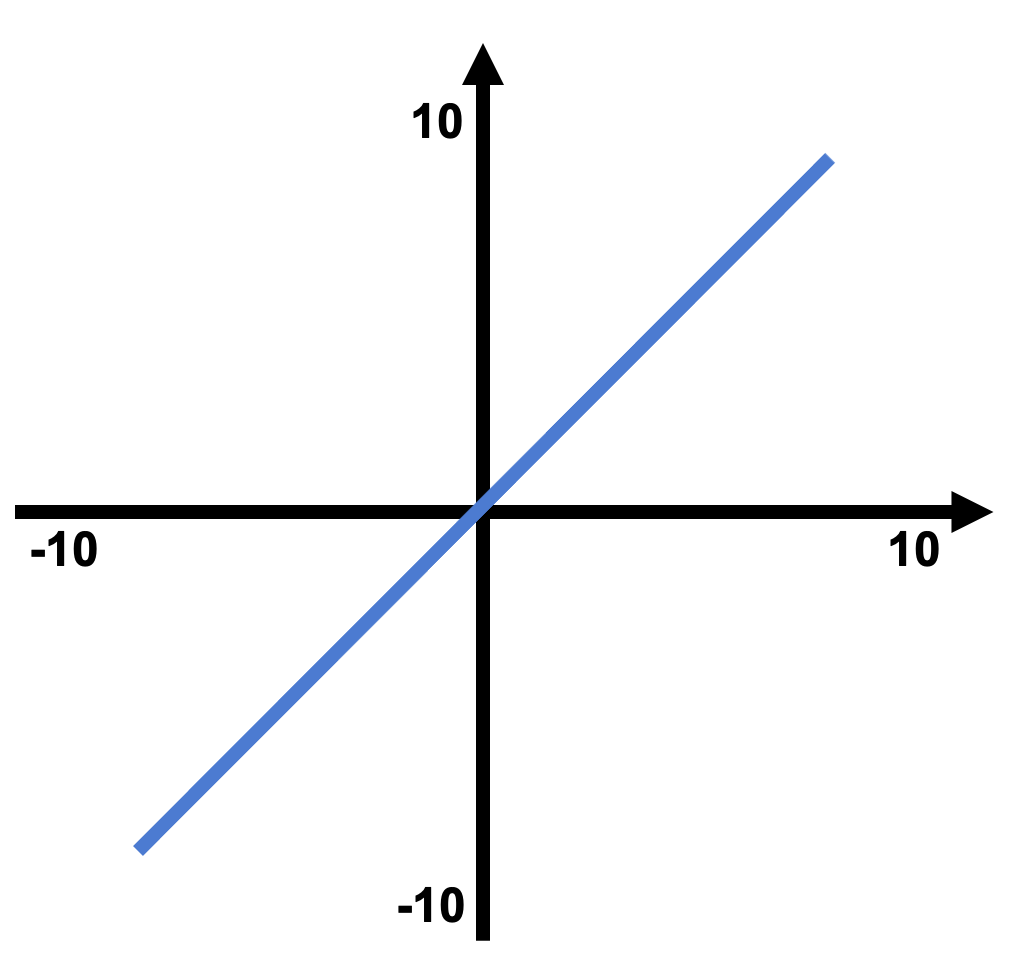
\includegraphics[width=0.3\textwidth]{ figures/estadoarte/lineal.png}} \hspace{10pt}
	        \subfigure[]{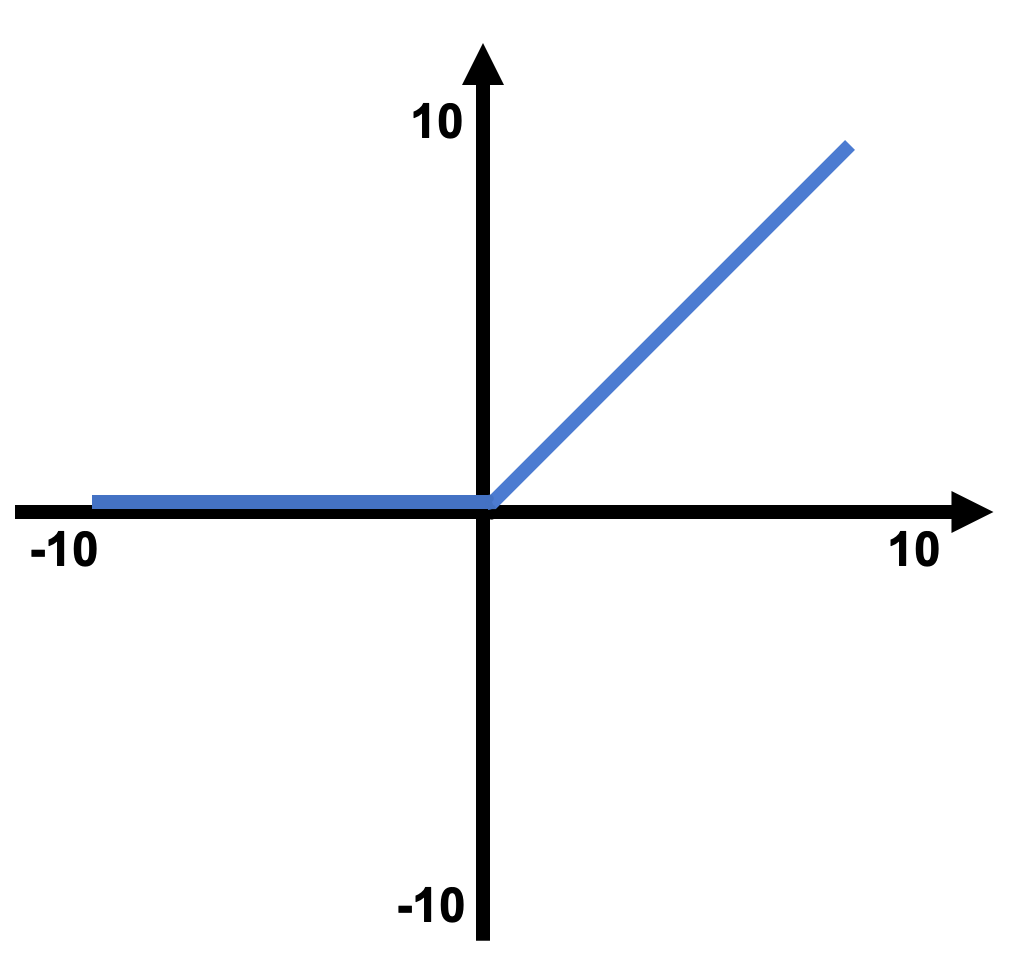
\includegraphics[width=0.3\textwidth]{ figures/estadoarte/relu.png}} \vskip\baselineskip
	        \subfigure[]{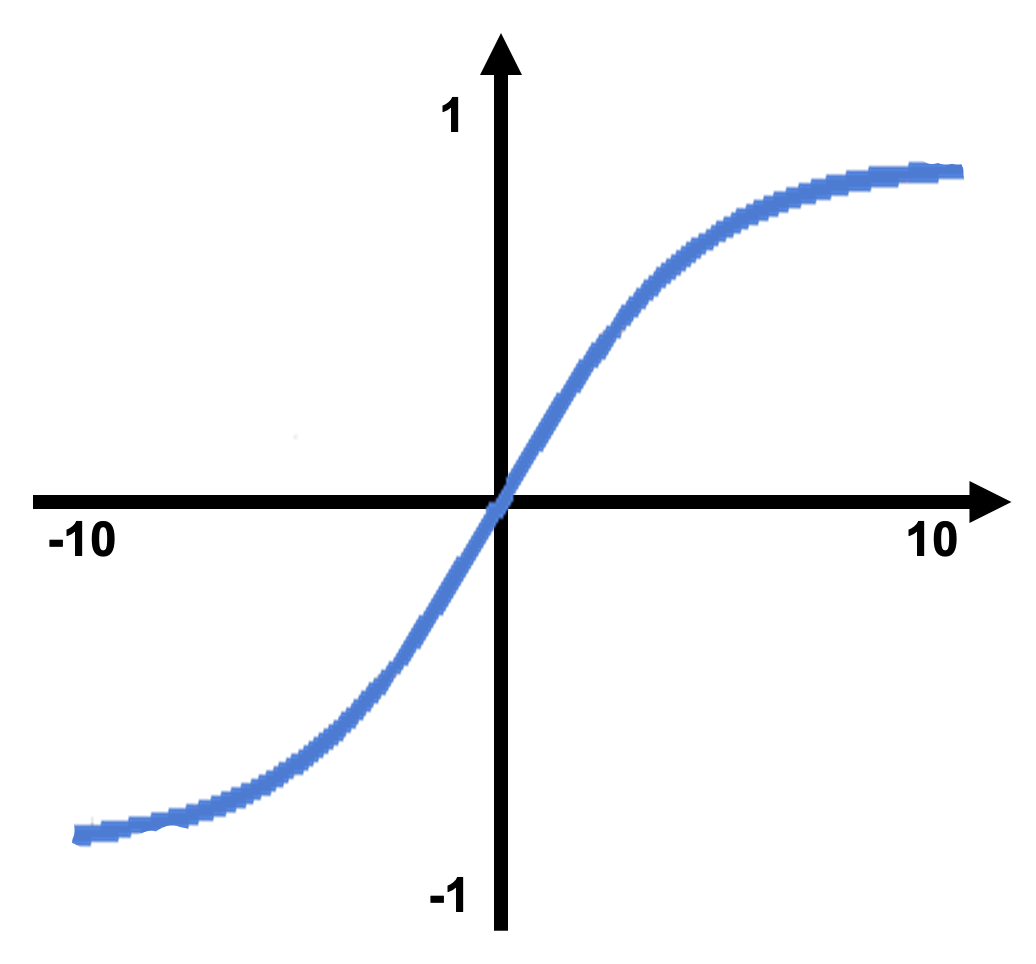
\includegraphics[width=0.3\textwidth]{ figures/estadoarte/tanh.png}}
	        \hspace{10pt}
	        \subfigure[]{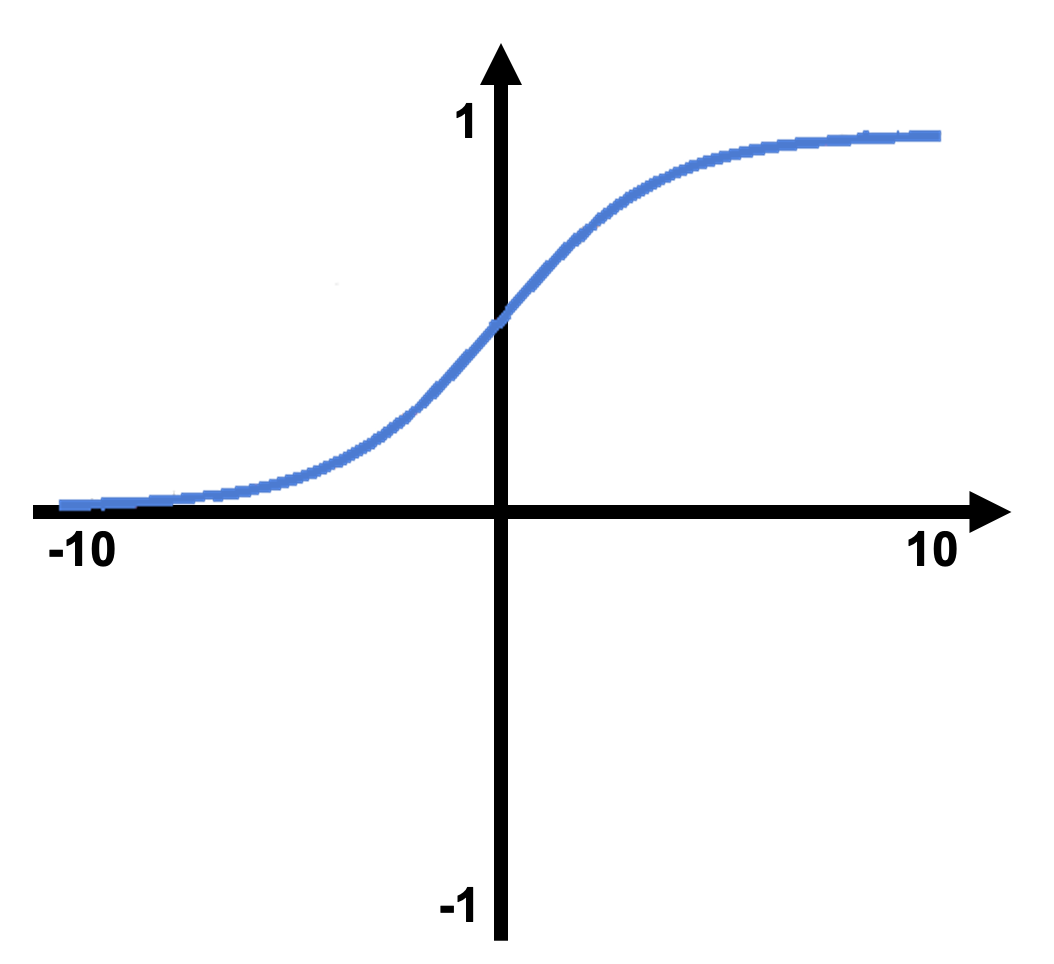
\includegraphics[width=0.3\textwidth]{ figures/estadoarte/softmax.png}}
	        \caption{Funciones de activación: (a)~Lineal, (b)~ReLu, (c)~Tanh y (d)~Softmax.}
			\label{fig.activacion}
		\end{center}
\end{figure}
\vspace{-10pt}

\subsection{Servidor Tamino}
Para la ejecución de los distintos procesos de este trabajo se ha utilizado un servidor Linux, Tamino, que está situado en el CPD de la ETSIT-URJC y pertenece a \textit{RoboticsLabURJC}. Las principales características de este servidor son:

\begin{itemize}
    \item \textbf{Procesador:} Intel(R) Xeon(R) CPU E5-2609 v4 @ 1.70GHz.
    \item \textbf{Número de núcleos:} 8 cores.
    \item \textbf{Memoria RAM:} 64GB.
    \item \textbf{GPU:} GeForce GTX 1080.
\end{itemize}

El uso de esta máquina ha permitido realizar entrenamientos más potentes así como el uso de conjuntos de datos más grandes.